\documentclass[10pt,a4paper,titlepage]{article}
\usepackage[utf8]{inputenc}

\usepackage{amsmath}
\usepackage{amsfonts}
\usepackage{amssymb}
\usepackage{graphicx}
\usepackage{float} % force figure to render inline location
\usepackage{enumitem} % apt install texlive-latex-extra 
\usepackage{anyfontsize} % custom fontsizes
\usepackage{titlesec} % custom section spacings
\usepackage{multirow} % merge table rows
\usepackage{vhistory} % revision table package
\usepackage{pdfpages}

\setlist[itemize]{noitemsep} % No spaces in itemize lists
\setlist[enumerate]{noitemsep} % No spaces in itemize lists
\setlist[description]{noitemsep} % No spaces in itemize lists
\titlespacing*{\subsubsection}{0pt}{8pt}{2pt}
\titlespacing*{\paragraph}{0pt}{3pt}{5pt}

\newcommand{\cpright}{\textsuperscript{\tiny\copyright}}

\setlength\parindent{0pt}

\begin{document}
	
	\begin{titlepage}
		
		\title{
			\fontsize{50}{12}\selectfont{\textsc{Lunar Rover}}\\
			\vspace{20pt}
			\fontsize{20}{12}\selectfont{\textsc{User Manual}}\\
			\vspace{10pt}
			\large{Software Engineering \& Project} \\
			\vspace{20pt}
			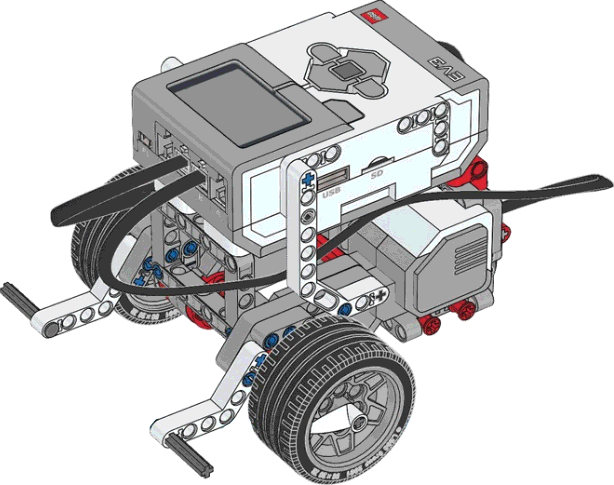
\includegraphics[width=200px]{title-page-ev3.png}					
		}
		\date{17/10/2017}
		\author{
			\bf{Team: PG-29} \\
			Benjamin Winding \\
			Kin Leong Lee \\
			Pavitterjeet Sidhu \\
			Phan Huy Nguyen \\
			Sean Hennessy \\
			Xiaoshan Chen \\
		}
		\maketitle
		
	\end{titlepage}
		 
	\tableofcontents	
	
	
	
	\section*{Revision History}	
	\label{revtable}	
	\begin{tabular}{|p{2.1cm}|p{2.5cm}|p{2cm}|p{4.1cm}|}		
		\hline 
		\textbf {Name} & \textbf{Date} & \textbf {Version} &\textbf {Summary of Changes} \\ 
		\hline 
		\hline 		
	\end{tabular}

	\newpage
	
	\section{GENERAL INFORMATION}
		\subsection{System Overview}
        This system consist two components a) The LEGO Mindstorm robot and the software to control it. The main aim of this system is to survey the specified area and safely return back to landing zone. The system is fully developed, tested and operational. GUI is also included in the system in-order to control the robot.
        The main features of this robot include
	\begin{itemize}
		\item Automatic survey of specified areas
		\item Remote control manual override and movement
		\item On-board obstacle avoidance mechanisms 
		\item No-go zone detection and avoidance
		\item Ability to return to the starting point or any point selected on mapped area.
\end{itemize}
   

        \subsection{Organization of the Manual}
        \subsubsection{User’s Manual v1.0.}
        \begin{itemize}
		\item Section 1 includes general information about the system
		\item Section 2 includes system summary
		\item Section 3 includes how to set up the system
		\item Section 4 includes how to use the system
\end{itemize}
        \subsection{Definitions, Acronyms and Abbreviations}
        \subsubsection{Definitions}
\begin{itemize}
\item Intellij IDE - Java(IDE) for developing computer software
\end{itemize}

\subsubsection{Acronyms}
\begin{itemize}
\item RMS - Robot Mapping System
\item OS - Operating System
\item JRE - Java Runtime Environment
\item IDE - Integrated development environment
\item NGZ - No Go Zone
\item SDD - Software Design Document
\item SRS - Software Requirements Specification
\item WDDM - Windows Display Driver Model
\end{itemize}

\subsubsection{Abbreviations}
\begin{itemize}
	\item min - minute
\end{itemize}
    \newpage    
	\section{SYSTEM SUMMARY}
		\subsection{System Configuration}
        \subsection{Data Flows}
        \subsection{User Access Levels}
        \subsection{Contingencies }
    \newpage
	\section{GETTING STARTED}
	\newpage
	\section{USING the SYSTEM}
	\newpage
	\section{Appendices}
		
	
\end{document}
